\chapter{Data Acquisition System\label{cha:chapter3}}
In this chapter, I would like to introduce TapSensing. TapSensing is a labeled data acquisition system designed to collect user generated taps with corresponding sensor readings. The system comprises of an iOS Swift and a Python Django server-side application. The chapter begins with a broader view on the system by explaining the overall system architecture and will then dive into it's individual components and implementation.

\section{Overall System Architecture}

The TapSensing application consists of two main components: the mobile and the server-side application. In brief, the mobile client provides the ability for a user to generate taps with corresponding motion sensor signals. For the data to be stored in a centralized manner, the server-side application provides HTTP endpoints as a gateway to the database. The architecture, as illustrated in figure \ref{fig:architecture}, consists of various components which are outlined in the following.

\begin{itemize}
  \item \textbf{Mobile application}: The iOS application provides interfaces for the user to generate taps and to label the data created. Furthermore, the application is capable of sending the acquired data to the server-side application. More features of the mobile application are presented in section \ref{sec:mobileapp}. % # TODO
  \item \textbf{NGINX}: For accepting and routing incoming HTTP requests, an NGINX reverse proxy/load balancer is used. The reverse proxy forwards the incoming requests to the server-side application and is capable of serving static content, such as images, HTML, CSS and JavaScript files of the form application.
  \item \textbf{Gunicorn}: Gunicorn\footnote{For more information on Gunicorn, visit \url{http://gunicorn.org/}.} is a Python Web Server Gateway Interface (WSGI) HTTP server which runs the source code of the backend application.
  \item \textbf{Backend Application}: The backend application provides authentication and persistence functionalities which are accessible through HTTP endpoints. More information on the backend application is to be found in section \ref{sec:backend}
  \item \textbf{PostgreSQL}: TapSensing uses a PostgreSQL\footnote{PostgreSQL is a general purpose and object-relational database management system.} database for storing the application state, user related information, the survey data and the retrieved tap and sensor information.
  \item \textbf{Form application}: The form application provides a web user interface where study participants can answer survey questions.
\end{itemize}

\begin{figure}[h!]
  \centering
  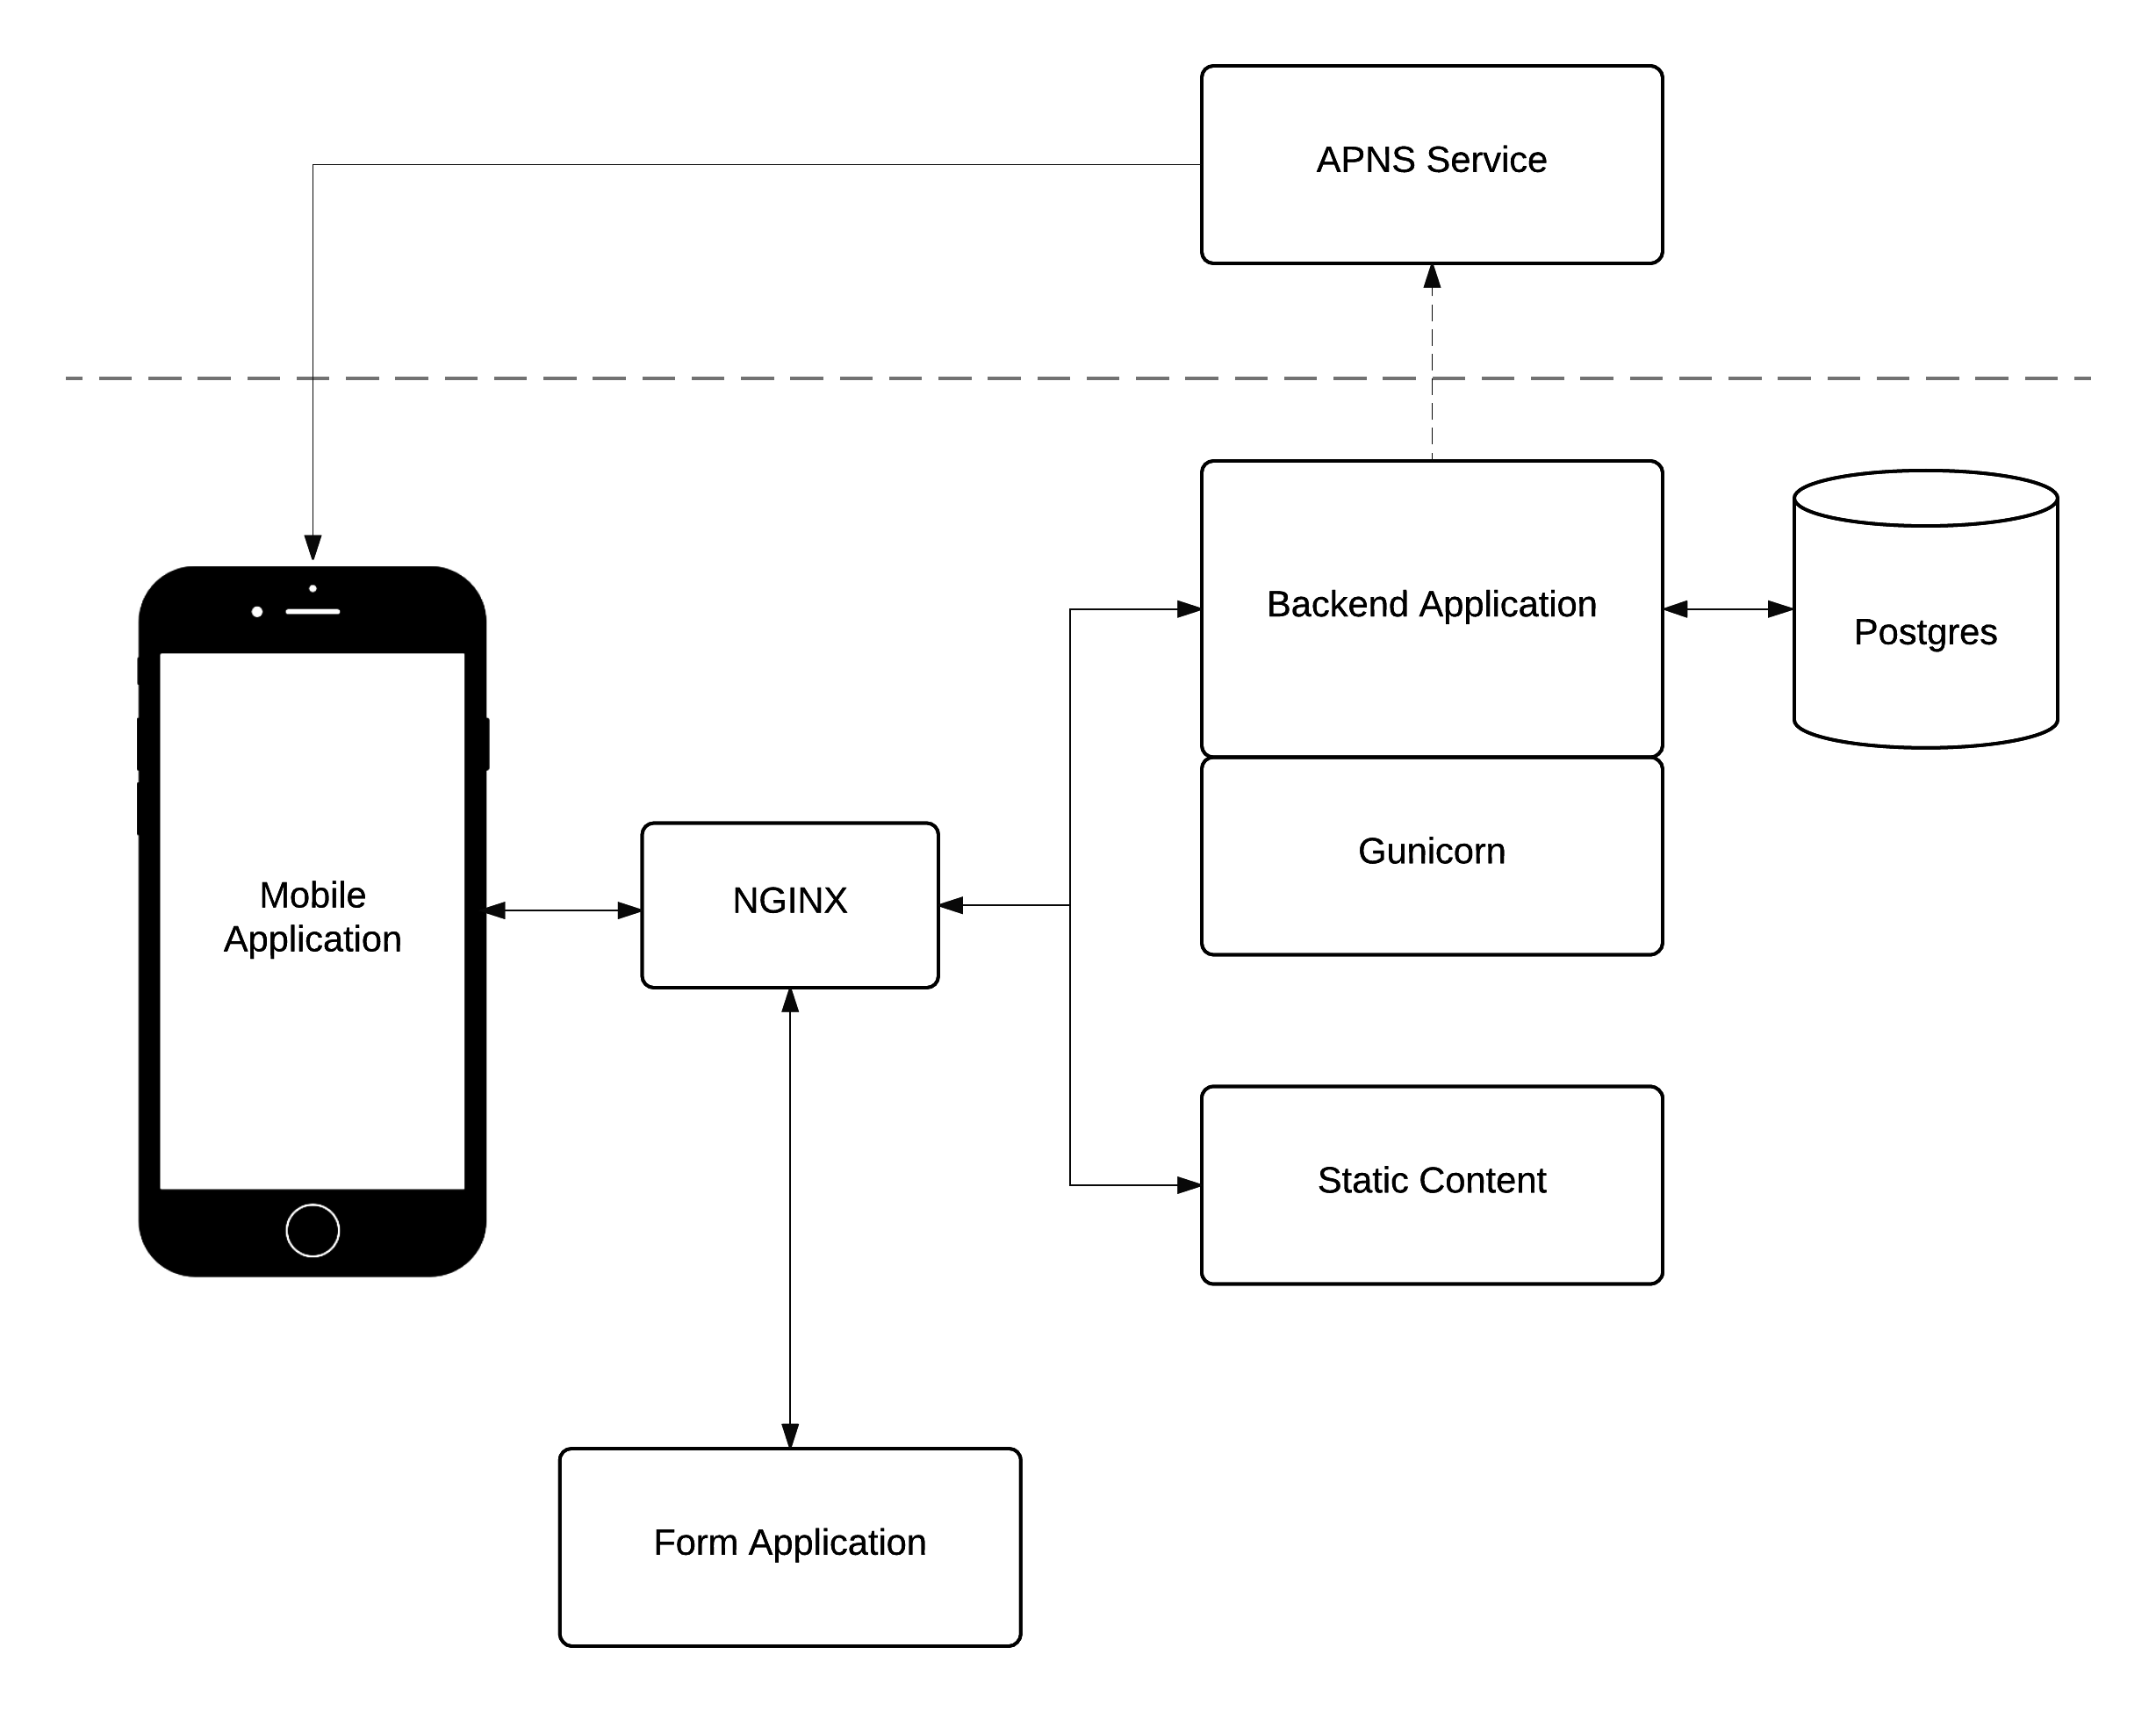
\includegraphics[width=1\textwidth]{architecture.png}
  \caption{The diagram shows the overall architecture of TapSensing.} \label{fig:architecture}
\end{figure}


% For the network requests containing the tap information which come from the mobile device to reach the backend, it must first pass through a reverse proxy. As reverse proxy we have chosen NGINX due to it's easy configurability. In this case, NGINX forwards requests to the TapSensing application and serves static files.\\
% The TapSensing backend is written upon the Python Django Framework\footnote{https://www.djangoproject.com/} which is being executed upon the gunicorn application server. Django uses a so-called ORM to perform transactions with the Database, which in our case is a PostgreSQL database.

\section{Mobile Application}
The TapSensing mobile application is a iOS App written in the Swift programming language designed to run on devices with iOS 10 and above. The main purpose of the application is to provide a user interface for subjects to create taps with accelerometer and gyroscope readings for the labeled data acquisition phase of the experiment.
\label{sec:mobileapp}

\subsection{User Interface}
\subsubsection{Login Screen}
When the application is opened for the first time, a login screen appears. As in standard login screens, the interface asks for credentials including username and password. Authenticating users, has the advantage, that the generated data can be mapped to individual users automatically.
\subsubsection{Start Screen}
During the trial the user is asked to generate taps once a day. In order to indicate if the user is eligible to perform a tap generation trial, the start screen shows a button that is either active or inactive. This switch depends on 4 distinct conditions:
\begin{figure}[h!]
  \centering
  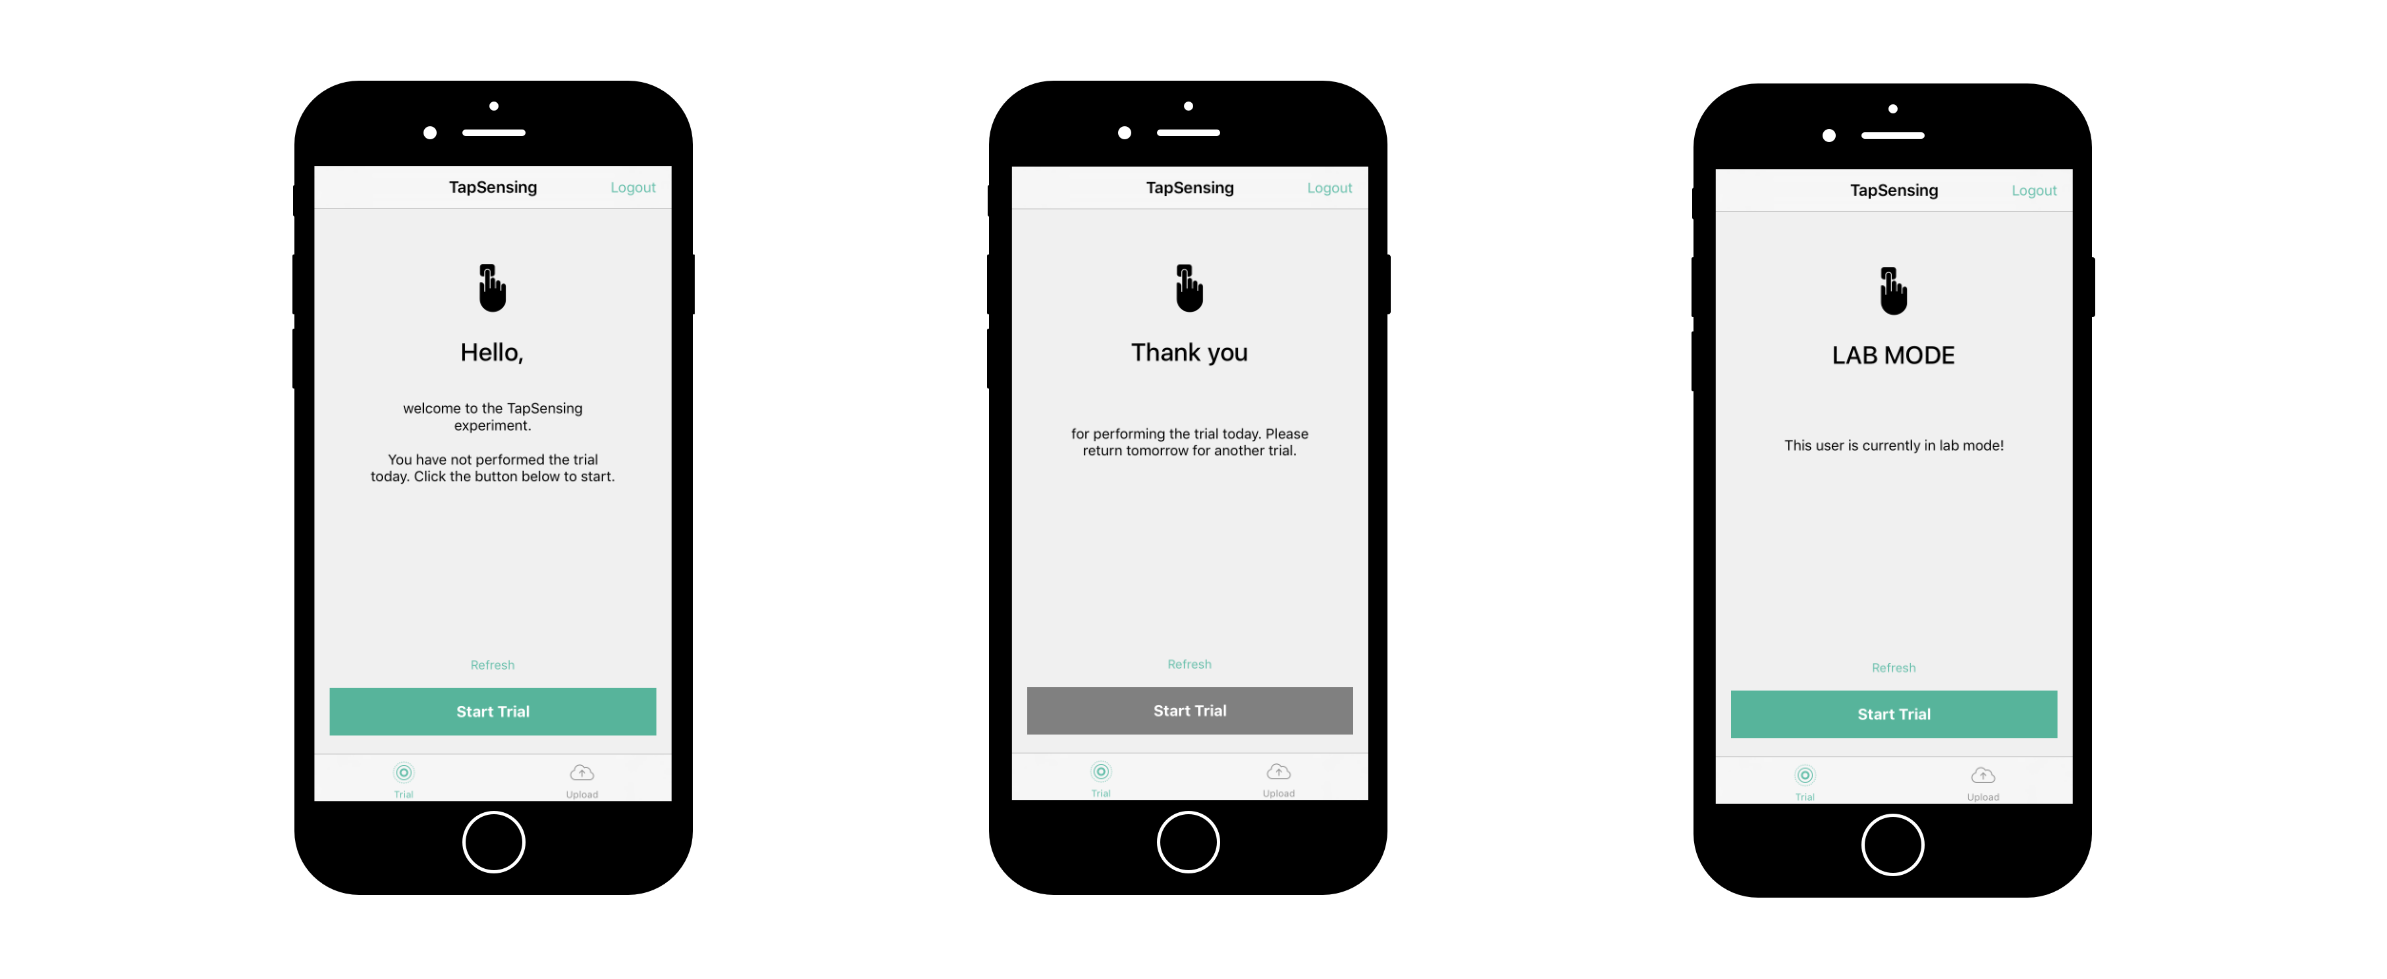
\includegraphics[width=0.8\textwidth]{iphones_startscreen.png}
  \caption{This figure shows the start screen in different configurations. On the left hand-side screenshot, the user has not performed a trial while the the middle image shows the screen where a trial has been performed. The right-hand side image shows the \textit{lab mode} where trails can permanently be performed.}
\end{figure}
When data is collected in the laboratory environment, the app is set to \textit{lab mode}. In \textit{lab mode} the button is always active and trials can be performed. When a user has not performed a trial today, the button is inactive. Consequently, when a user has already performed a trial on a specific day, the button is inactive and a further trial can only be performed on the following day. Once all field trials are performed, the app confirms that all data is collected and the button remains inactive.
\subsubsection{Tap Input Screen}
To acquire individual user taps the mobile application offers a user interface where buttons are aligned in a grid shape structure. The structure is calculated based on a specific configuration set where the amount the vertical and horizontal buttons in the interface can be set. Figure \ref{fig:grid} shows the interface, where 4, 12 and 20 distinguishable buttons are configured.
\begin{figure}[h!]
  \centering
  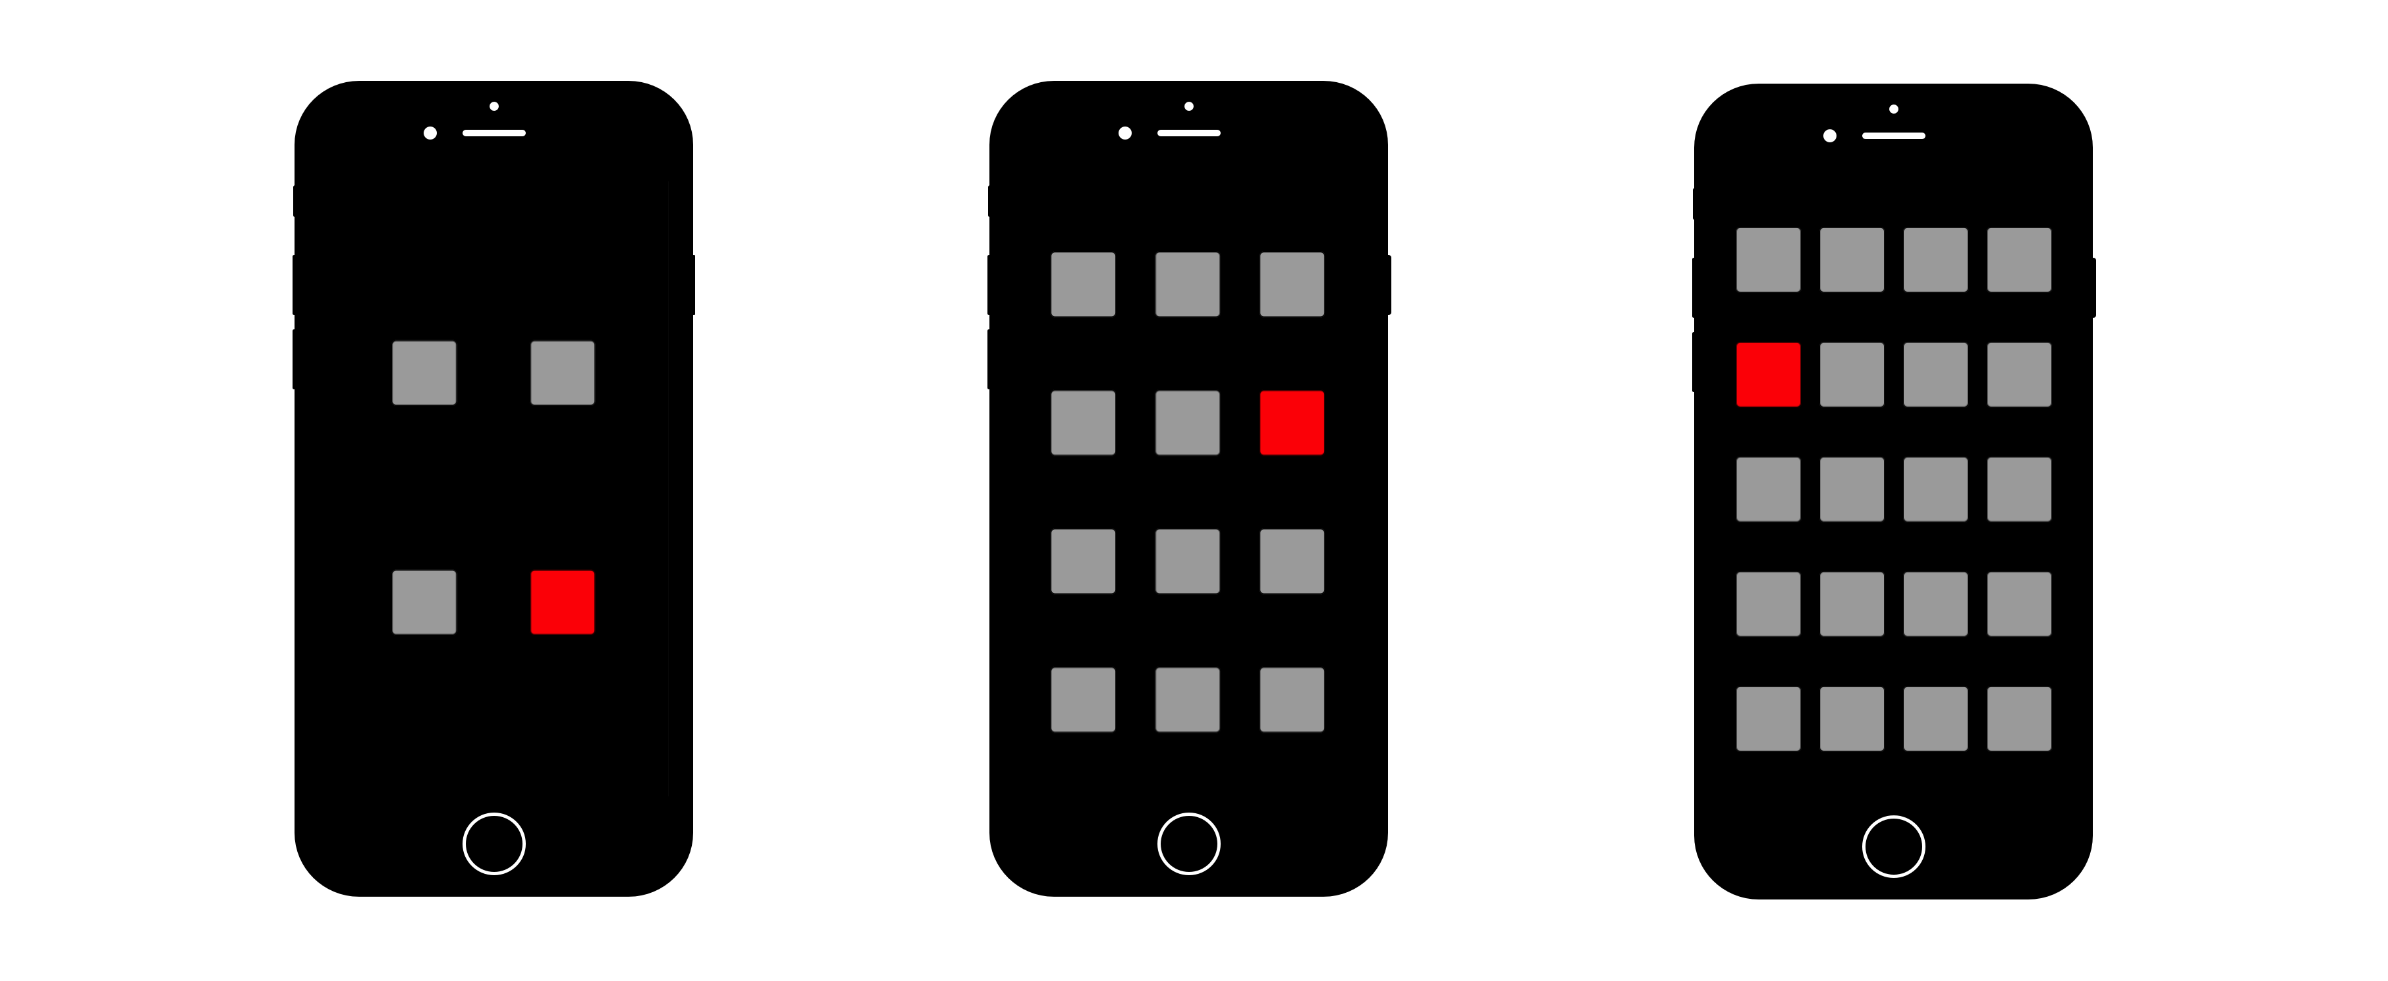
\includegraphics[width=0.8\textwidth]{grids_iphone.png}
  \caption{The figure shows the tap input user interface with buttons aligned in a grid shape structure. The leftmost structure offers 4 buttons, the middle offers 12 buttons whereas displays 20 distinguishable buttons.}\label{fig:grid}
\end{figure}
For the user to tap on every location of the screen exactly once, a red button indicating the next button to tap is highlighted guiding the user through the interaction process. While the user is tapping the grid, the gyroscope and accelerometer information is recorded. After all buttons gave been tapped, either a new grid is loaded or the tap acquisition phase ends proceeding with the question interface.

\subsubsection{Questions Screen}
\begin{figure}[h!]
  \centering
  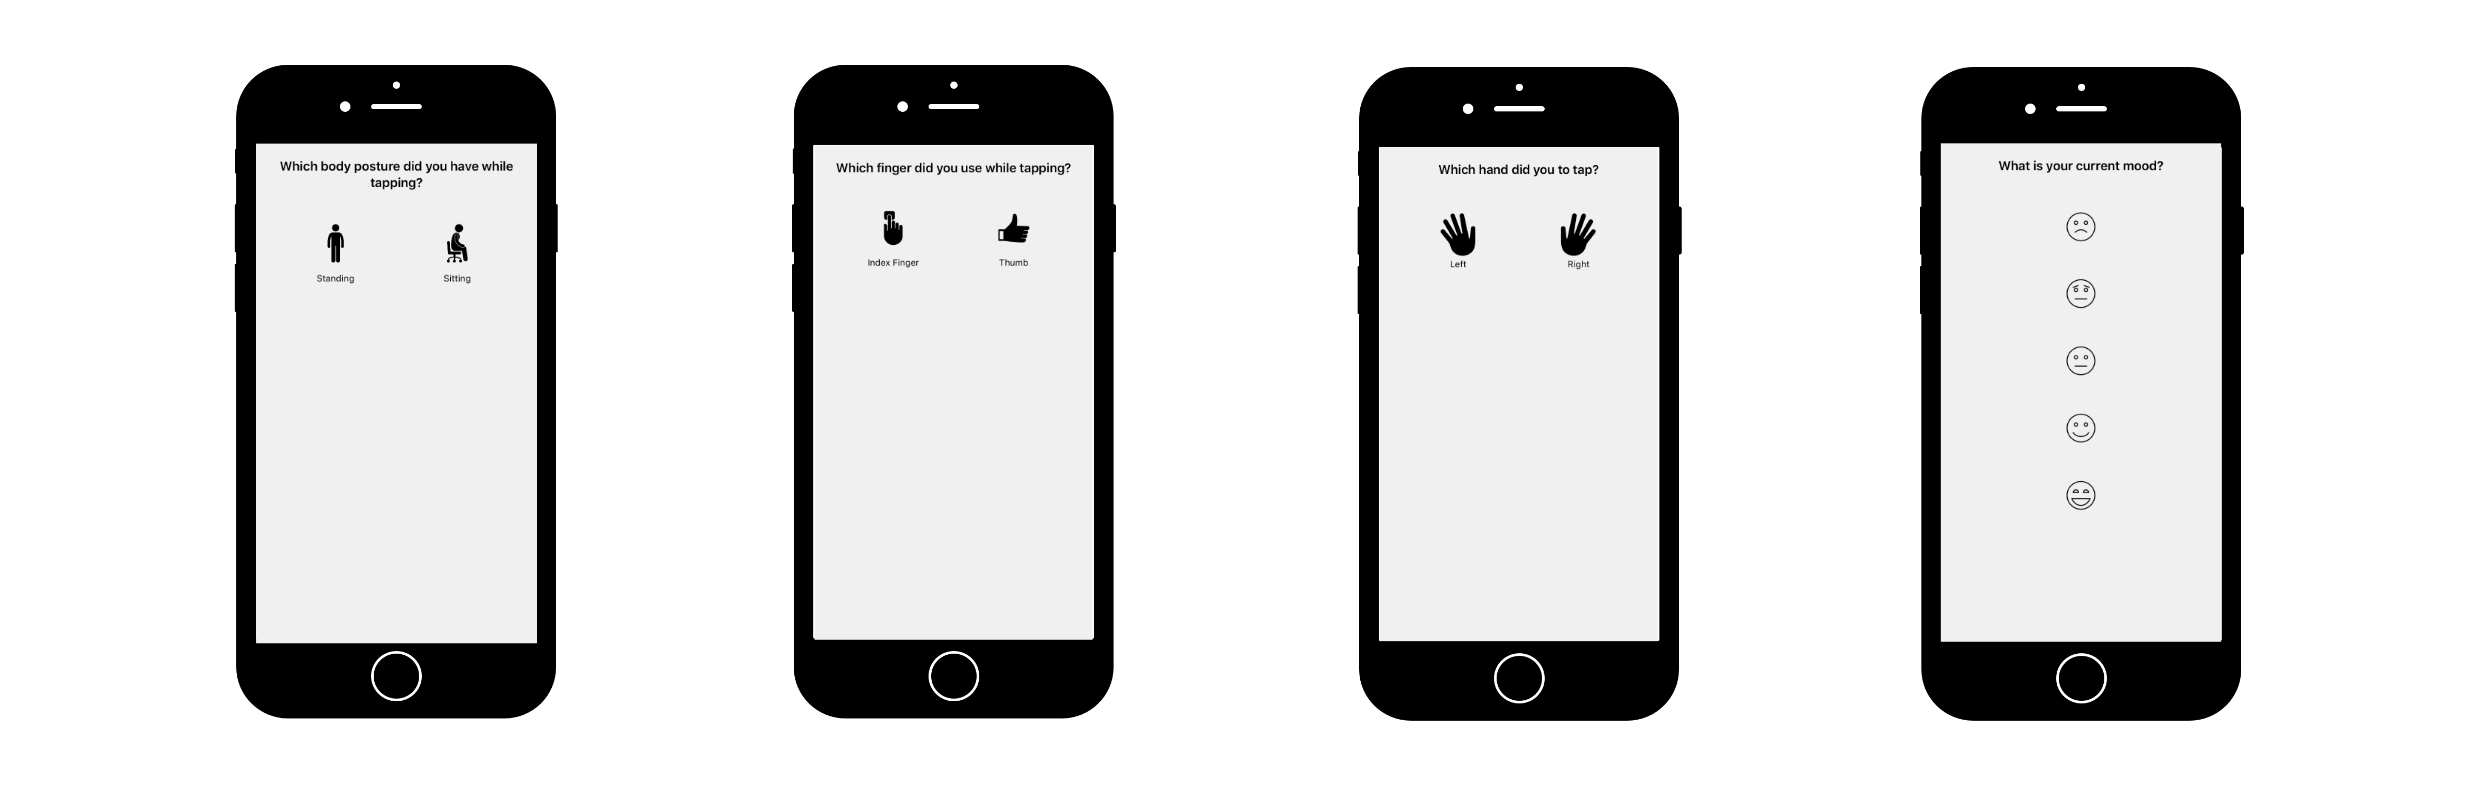
\includegraphics[width=1\textwidth]{questions_iphone.png}
  \caption{The figure displays question views with icons as answer possibilities.}
\end{figure}

To label the data acquired in the tap input interface, the application provides screens for the user to answer several questions. These question regard the body posture, input modality and the mood in which the user has generated the taps. In the table \ref{table:questions} below the questions asked with corresponding answer choices are to be found.


\begin{table}
  \centering
  \begin{tabular}{| l | l | l | l |}
  \hline
  \textbf{Question} & \textbf{Answer Choices} \\ \hline
  Which body posture was used during the interaction ? & Standing, Sitting \\
  Which finger did you use while tapping? & Index Finer, Thumb \\
  Which hand did you use to tap? & Left, Right \\
  What is your current mood? & 1 - 5 \\
  \hline
  \end{tabular}
  \caption{The Table shows the questions asked in the question view.}\label{table:questions}
\end{table}

To enable fast interactions, each answer possibility to a question is represented in the interface with an icon. Once an icon has been pressed, the application transits to the next question until all questions have been answered.

\subsubsection{Upload Screen}
After all taps and questions are gathered, the acquired data is sent to the server. The interface at this points displays a spinning wheel for the user to acknowledge that the mobile phone is processing the data. In case an upload fails, the application provides a manual upload screen, where past sessions can be uploaded.

\subsection{Implementation Notes}
\subsubsection{Obtaining Sensor Information}
In order to access the gyroscope and the accelerometer, Apple provides a high-level API\footnote{An Application Program Interface is a set of rules and subroutines provided by an application system for the developer to use. The following link leads to the Core Motion API documentation: \url{https://developer.apple.com/documentation/coremotion/} } for accessing the device's sensors: \textit{Core Motion}. Core Motion provides motion and environmental related data from sensors including accelerometers, gyroscopes, pedometers, magnetometers, and barometers in easy to use manner.

Sensor values can either be accessed as proceeded including aggregations of the values or as raw version. For TapSensing, raw values are recorded to avoid any form of bias. The update interval can be configures at ranges from $10$Hz - $100$Hz. Higher update-rates are possible but are not ensured to be processed in real-time by the device. For TapSensing, the update rate is configured with the highest (safe) value possible. This ensures that tap patterns are captured with high resolution in order to make a classification easier.
\subsubsection{Local Persistence}
It is possible that a session upload fails due to lack of internet access or another reason. Due to this, the application stores all session information and sensory data in it's local SQLite database. For local persistence Apple provides it's own framework called \textit{Core Data} which is extensively used in TapSensing. Once the data has been successfully received by the backend, the data is deleted from the local database.
\subsubsection{Ensuring data consistency}
Sending all collected data in a single HTTP-request results in the sent package being too large for the server-side system to process. For this reason, the data is split up into packages of 300 objects per request. To send these requests in an asynchronous manner, the \textit{Promise}\footnote{Promises are a software abstracting for dealing with asynchronous computation. Promises are objects that may produce a value at some point in the future.}\cite{Liskov:1988:PLS:53990.54016} library \textit{Hydra}\footnote{\url{https://github.com/malcommac/Hydra}} is used.

During an upload phase, packages are sent in a sliding window approach. Packets are sent three at a time until all packages have been acknowledged by the server-side application. For each transmitted package, the server responds with the amount of data objects contained within the request. The mobile client can therefore track the amount of packages transmitted to ensure that all data has been transmitted successfully.
If one packet fails to arrive, the package is resent with an exponential back-off.
\subsubsection{Push Notifications}
TapSensing is registered with the Apple Push Notification Service allowing the application to receive push notifications. Notifications are used to remind the user during the field study, that he has to take part in the study.
\subsubsection{Distribution}
Installing iOS applications that are not uploaded to the Apple App Store, requires each device to be registered in the Apple Developer Portal with the smartphone's serial number. To avoid this, the application has been uploaded to the App Store enabling an easy distribution.

\section{Backend application}
The purpose of the backend application is to provide persistence functionalities for the acquired taps generated with the mobile application. The application is written on top of the Django\footnote{\url{https://www.djangoproject.com/}} web application framework and the Django REST framework\footnote{\url{http://www.django-rest-framework.org/}}.

\label{sec:backend}
\subsection{HTTP Endpoints}
\label{sec:endpoints}
For the purpose of interoperability the network communication from the mobile application and the forms application to the server-side application is done via HTTP Requests in the JSON\footnote{JSON (JavaScript Object Notation)\cite{ietf-jsonbis-rfc7159bis-04} is a lightweight data-interchange format.} format. The endpoints listed below represent tiny logic components that can be called from an external client.

\begin{table}[h!]
  \begin{tabular}{|p{2cm}|p{4cm}|p{8cm}|}
  \hline
  \textbf{HTTP \newline Method} & \textbf{URL} & \textbf{Description} \\ \hline
  POST & /login & Provides login functionalities for the mobile client. This method returns an authentication, that is used for further requests to authenticate the user.\\
  \hline
  POST & /session & Provides upload functionality for a session data objects.\\
  \hline
  POST & /touchevent & Provides upload functionality for touchevent data objects.\\
  \hline
  POST & /sensordata & Provides upload functionality for a sensordata data objects.\\
  \hline
  POST & /apns & Retrieves the Device's APNS token. This is required to send push notifications to the users.\\
  \hline
  GET & /trial-settings & Provides the configuration for the tap input view. Here, the amount of buttons and the amount of grid repetitions that are to be performed in a single session can be defined.\\
  \hline
  POST & /survey & Provides upload functionalities for the survey form application.\\
  \hline

  \end{tabular}
  \caption{The table shows all HTTP endpoints of the server-side application.}\label{table:endpoints.}
\end{table}

\subsection{Data Model}
TapSensing's data model reflect the schemas that are used in the PostgreSQL database. As seen in figure \ref{fig:erdiagram}, the data model consists of 4 data objects that I will describe in this section:

\begin{itemize}
  \item \textbf{User}: The user model is inherited by the Django's user model\footnote{For more information on the Django user model, the following URL leads to the model's documentation: \url{https://docs.djangoproject.com/en/1.11/ref/contrib/auth/}}. The user model is used for authentication and persisting the authentication token. The other models described in this section are connected to the user model through a foreign key relation to identify the user associated with the data object.
  \item \textbf{Session}: The session data object holds all information associated with the user's trial. This includes the data collecting in the ``labeling part''\footnote{The ``labeling part refers to the question views, where additional information on the data acquired is collected'''} of the application such as the hand used, the body posture and the typing modality. In addition, information is stored such as device infos and if the session took place in a laboratory or field environment.
  \item \textbf{Touchevent}: The touchevent data object stores information regarding the ``ground truth'' of the user generated tap including the exact x and y coordinates, timestamp and an identifier of the specific grid rectangle tapped in the tap input view. Furthermore, it is noted if the user hit a specific rectangle and if the event is a touch-down or touch-up event.
  \item \textbf{Sensordata}: The sensordata data object captures all information obtained by the gyroscope and accelerometer of the mobile device. To differentiate between accelerometer and gyroscope values, the data object includes a type field. In addition, the model captures the timestamp and the 3-sensor components (x, y, z) of the individual sensors.
\end{itemize}

\begin{figure}[h!]
  \centering
  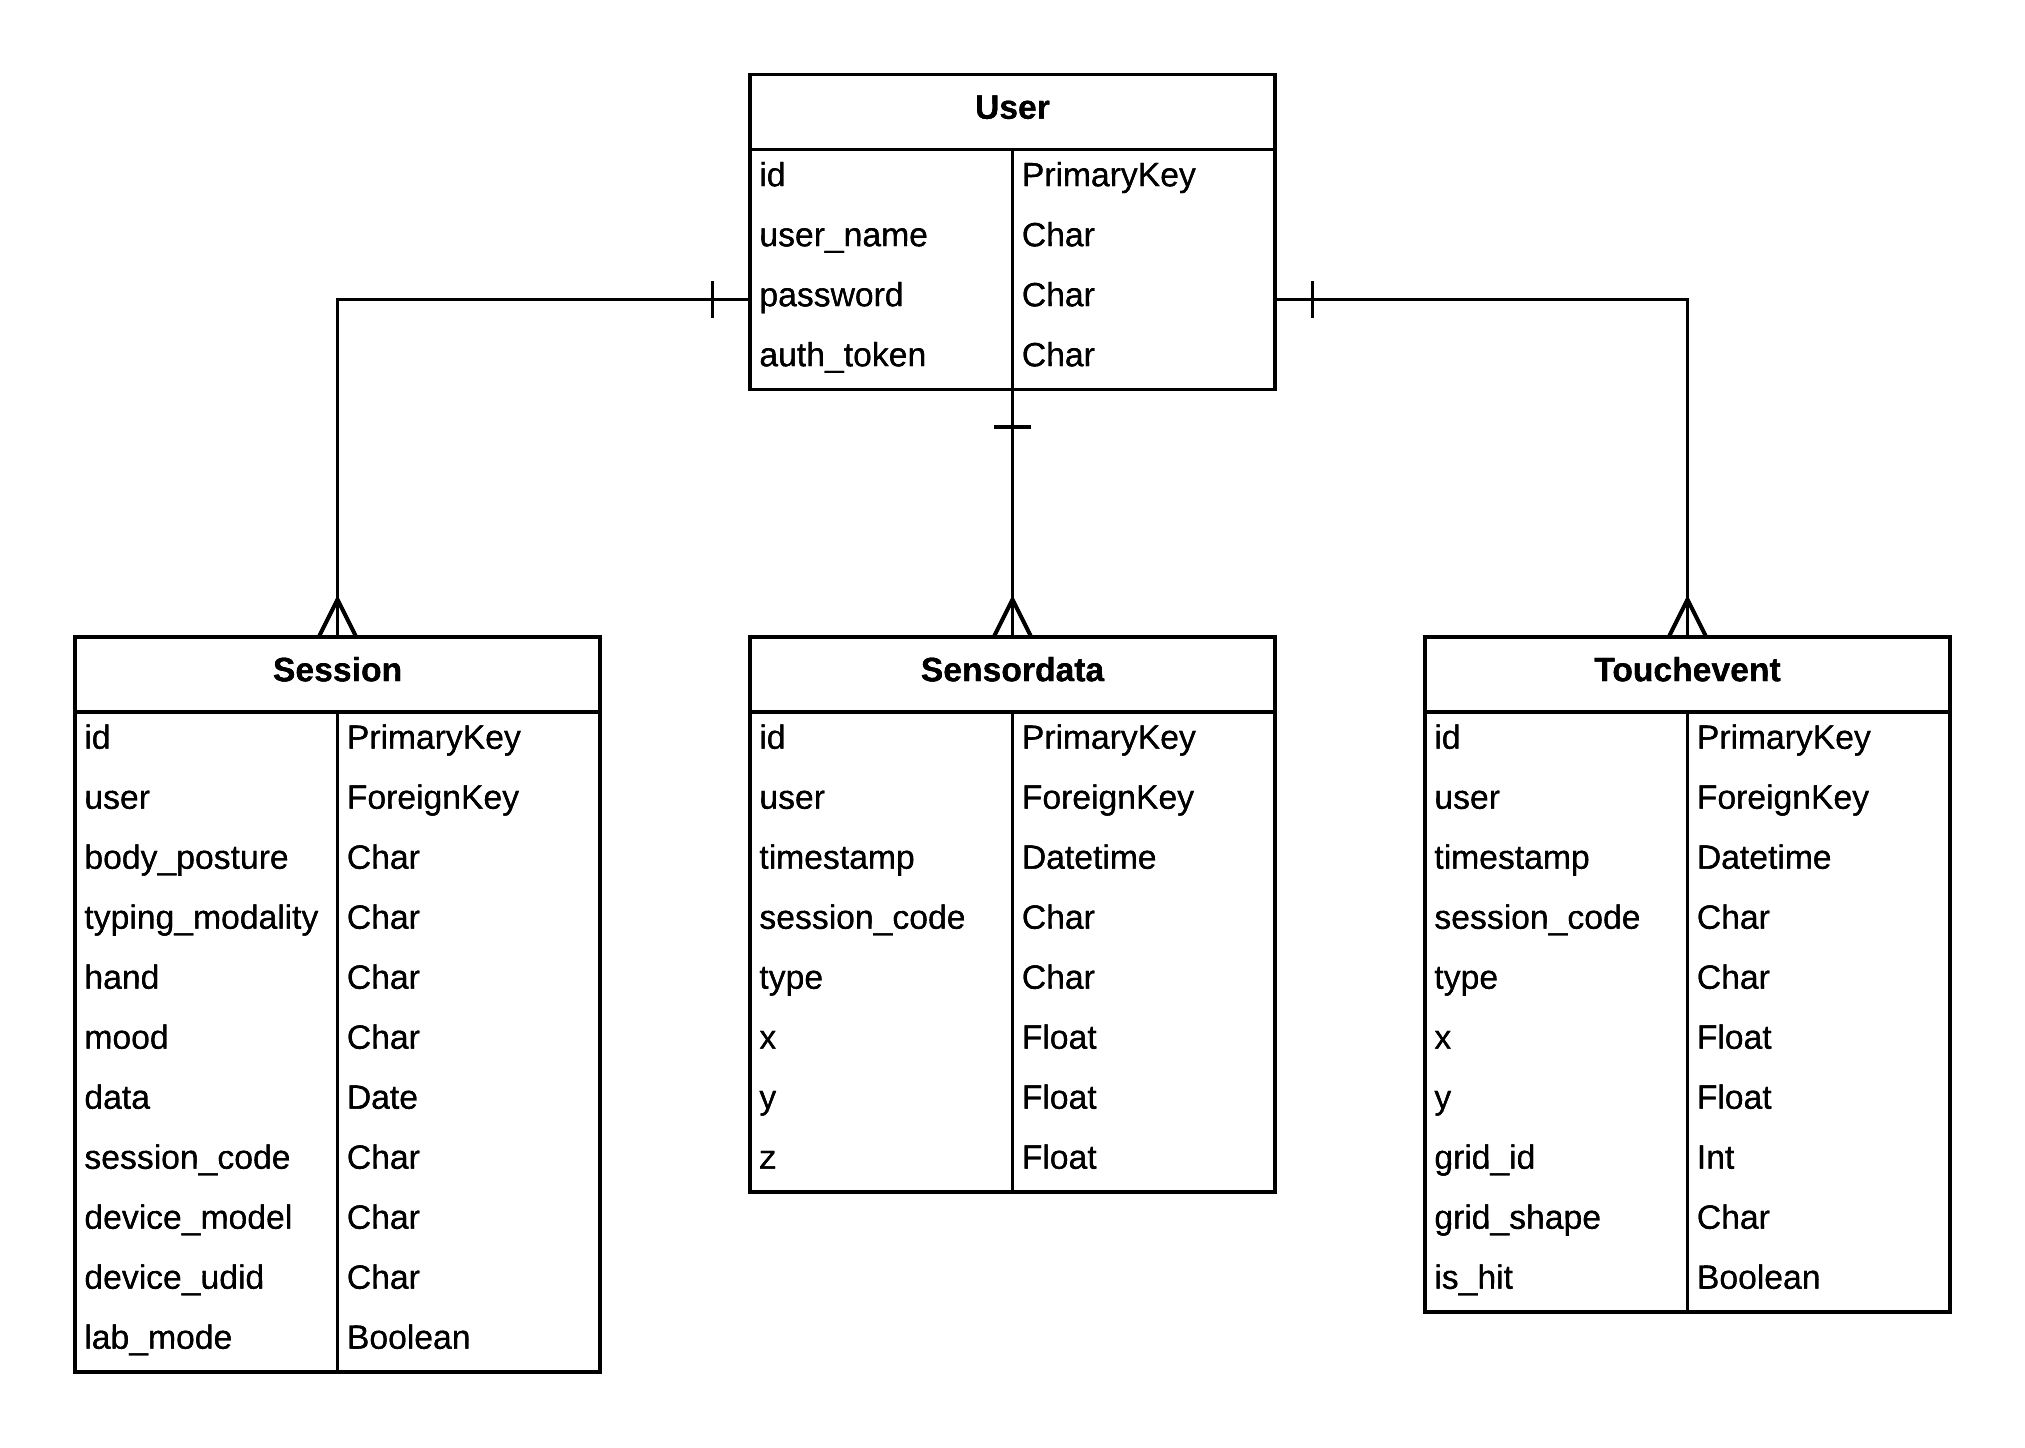
\includegraphics[width=1\textwidth]{datamodel1.png}
  \caption{The diagram shows TapSensing's data model with the user, session, sensordata and touchevent data object.} \label{fig:erdiagram}
\end{figure}

% An additional model was created for the survey application.

% \begin{figure}[h!]
%   \centering
%   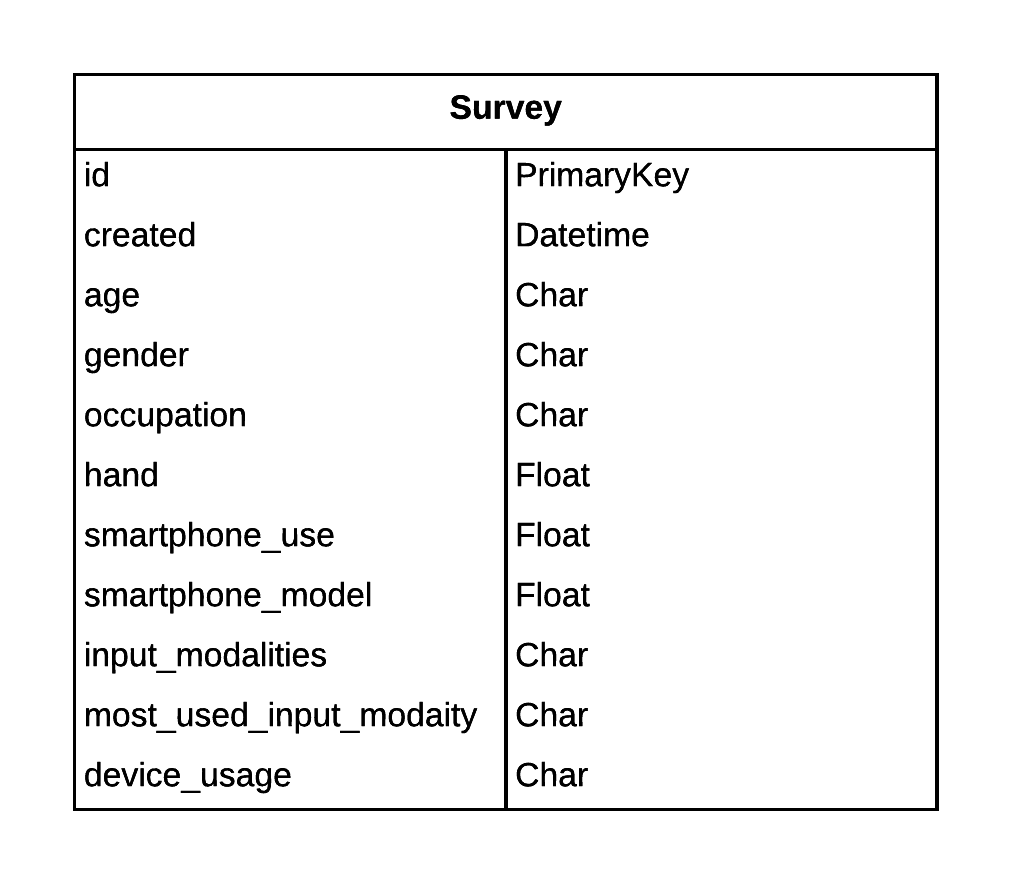
\includegraphics[width=0.4\textwidth]{datamodel2.png}
%   \caption{The diagram shows TapSensing's data model with the user, session, sensordata and touchevent data object.} \label{fig:erdiagram}
% \end{figure}

\subsection{Implementation Notes}
\subsubsection{Authentication}
The authentication mechanism implemented in TapSensing is based on a standard token authentication scheme. This allows the association of an incoming request with a set of identifying credentials, which is - in this context - the user the request came from. In order to obtain an authentication token, the mobile application sends the login credentials of a user including username and password to the login endpoint\footnote{The login endpoint is described in section \ref{sec:endpoints}.}. When the credentials have been checked for validity, the endpoints returns an authentication token in the following format:
\begin{minted}[tabsize=4]{js}
{ "token": "Token 3acc6c2a58723e2f1579d4526add2511f6a0a525" }
\end{minted}
The token is then added to the HTTP-request in the ``Authorization'' header to authenticate the user.

\subsubsection{Push Notifications}
As a previous study has shown that push notifications greatly enhance user participation \cite{pushNot} during a mobile field study, notifications are sent on a daily basis reminding the participants to take action. In the same study\cite{pushNot}, passive notifications - notifications without sound - have been seen to futhermore impact the participation. Following these assumptions, a push notification strategy has been designed combining notifications with and without sound. Figure \ref{fig:push-notifications} shows this implemented strategy with corresponding trigger times.

% \begin{figure}[h!]
%   \centering
%   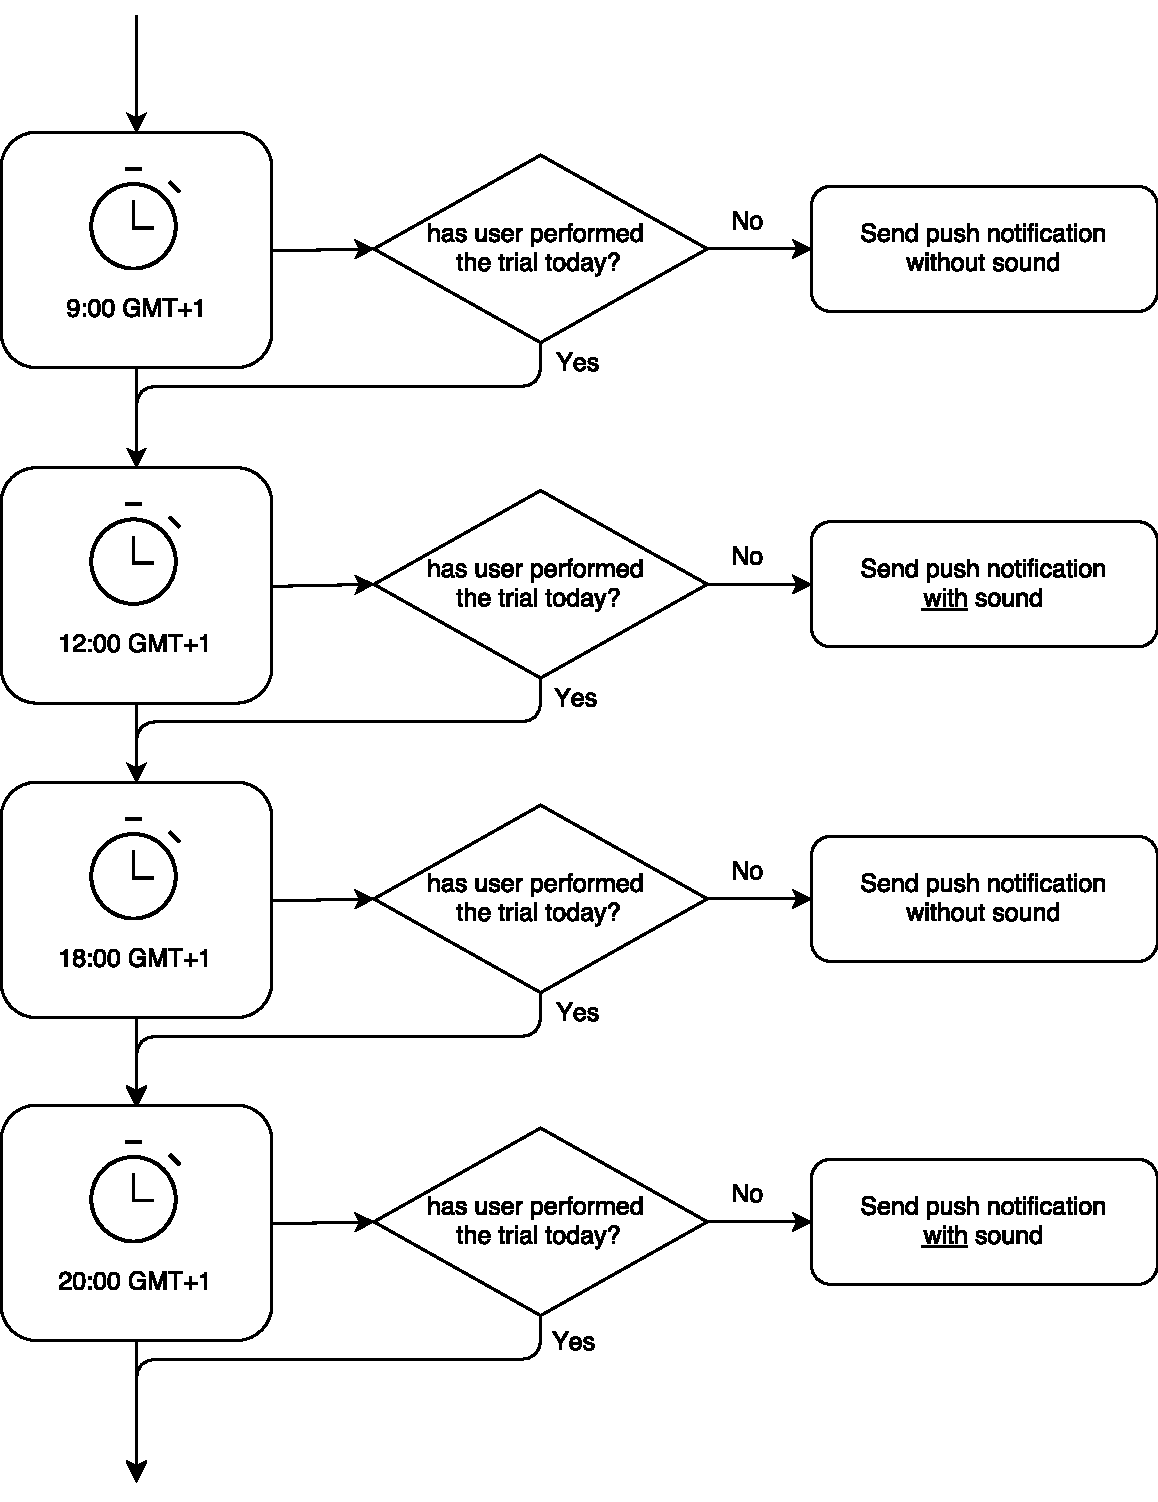
\includegraphics[width=0.5\textwidth]{push_notifications.pdf}
%   \caption{The diagram shows the implemented push notification strategy.} \label{fig:push-notifications}
% \end{figure}
\begin{center}
  \begin{tabular}{ | l | p {9cm} | l |}
  \hline
  Time & Message & Sound \\ \hline
  9:00 GTM+1 & Good Morning. This a friendly reminder to take part in the tapsensing study today. & inactive \\
  12:00 GTM+1 & Tapping is a lot of fun. Have you tapped the buttons today? & inactive \\
  18:00 GTM+1 & I know your day is busy, but don't forget to take part in the study. & inactive \\
  21:00 GTM+1 & You have not taken part in the study today. Please do it now. & active \\
  \hline
  \end{tabular}
  \captionof{table}{The table shows the push notifications strategy with individual notifications sent.}\label{table:anns}
\end{center}

The interaction with the APNS service has been implemented using the Django package \textit{django-push-notifications}\footnote{\url{https://github.com/jleclanche/django-push-notifications}}. It is used to provide mechanisms to register devices as well as to send notifications. To trigger the notifications at specific times unix cronjobs are executed.
\subsubsection{Backups}
To prevent data loss, the PostgreSQL database is backed up via a unix cronjob every evening. The database dumps are sent automatically to Amazon Web Services S3 Bucket.
\subsubsection{Deployment}
The server-side application with the NGINX reverse-proxy and a gunicorn WSGI application server has been deployed on a Ubuntu 14.04 virtual environment. The server comprises of 1GHz of shared CPU and 1 GB RAM.